
\chapter{Entwicklung}

\section{Konzeprionierung Observer-Modul}
\label{Grundger\"ust_ObserverModul}


\newpage
\section{Interruptgesteuertes Lesen und Schreiben}
\label{Interruptgesteuertes_Lesen&Schreiben}


\newpage
\section{Debugging-Methoden: Hardware- vs. Software-Breakpoints}
\label{Hardware_VS_Software_Breakpoints}

Im Kontext der Fehlersuche und Programmanalyse in Embedded Systems stellen \Fachbegriff[Bezeichnet in der Softwareentwicklung eine vom Entwickler bewusst gesetzte Unterbrechung im Programmablauf, die typischerweise zur Laufzeit-Debugging-Zwecken verwendet wird. Beim Erreichen dieses Punkts wird die Ausf\"uhrung des Programms angehalten, sodass der aktuelle Zustand (\zB Variableninhalte, Stack, Speicher) analysiert werden kann.]{Breakpoints} ein fundamentales Werkzeug dar. Sie erm\"oglichen es, die Ausf\"uhrung eines Programms an einer vordefinierten Stelle zu unterbrechen, um den internen Zustand des Systems zu inspizieren. Grunds\"atzlich lassen sich zwei prim\"are Arten von Breakpoints unterscheiden: Software-Breakpoints und Hardware-Breakpoints, deren Implementierung und Eigenschaften sich signifikant unterscheiden.

Software-Breakpoints werden zur aktiven Laufzeit des Programms durch einen direkten Eingriff in den ausf\"uhrbaren Code im Speicher des Mikrocontrollers realisiert. An der Zieladresse wird hierbei die urspr\"ungliche Programminstruktion tempor\"ar durch eine Breakpoint-Instruktion oder einen Trap-Befehl ersetzt, der einen Software-Interrupt oder eine Exception ausl\"ost. Sobald der Programmz\"ahler diese modifizierte Stelle erreicht, unterbricht der Mikrocontroller den normalen Programmfluss der Programmzähler stoppt und eine Debug-Routine wird ausgeführt. Der \Fachbegriff[Ein Werkzeug zur schrittweisen Ausf\"uhrung und Analyse von Programmen. Es erlaubt das Setzen von Haltepunkten, das \"uberpr\"ufen von Speicherinhalten und das Nachvollziehen von Kontrollfl\"ussen zur Fehlersuche und -behebung.]{Debugger} kann diesen Zustand erkennen, die urspr\"ungliche Instruktion wiederherstellen und dem Entwickler die Kontrolle \"ubergeben. Durch diesen Mechanismus sind Software-Breakpoints hochflexibel und k\"onnen an nahezu jeder beliebigen Stelle im beschreibbaren Code-Speicher (wie RAM oder FRAM) gesetzt werden.

Die Vorteile des softwarebasierten Ansatzes liegen prim\"ar in der M\"oglichkeit, eine praktisch unbegrenzte Anzahl von Breakpoints im System zu verwenden, sowie in den geringen Anforderungen an zus\"atzliche, dedizierte Hardwarekomponenten auf dem Zielsystem selbst. Die grundlegende F\"ahigkeit, Interrupts oder Exceptions zu behandeln, ist hierf\"ur ausreichend. \Zitat[Kap. 4.7.16]{ti:CCS}

Gegen\"uber den Software-Breakpoints bieten hardwarebasierte Breakpoints den Vorteil, dass sie Programmunterbrechungen auch in solchen Speichersegmenten erm\"oglichen, die schreibgesch\"utzt sind (z.B. ROM oder spezifisch gesch\"utzte Flash-Bereiche). Ein weiterer entscheidender Vorteil ist ihre Nicht-Intrusivit\"at: Da keine Modifikation des Programmcodes stattfindet, werden weder die Konsistenz des Codes im Speicher noch das pr\"azise Echtzeitverhalten (Timing) des Programms durch den Breakpoint-Mechanismus selbst beeinflusst. \Zitat[Kap. 4.7.16]{ti:CCS}, \Zitat[S. 54, Kap. 4.3]{ti:spru296}

Um dies jedoch zu erreichen, ben\"otigen Hardware-Breakpoints ein dediziertes Hardwaremodul innerhalb des Mikrocontrollers. Im Falle der MSP430-Mikrocontrollerfamilie ist dies das \NeuerBegriff{Embedded Emulation Module (EEM)} \Zitat[S. 569, Kap. 21]{ti:slau272d}. Dieses Modul beinhaltet spezielle Hardwareregister, typischerweise Adresskomparatoren, welche die Speicheradresse des Befehls halten, an welcher bei \"ubereinstimmung mit dem Programmz\"ahler ein Breakpoint ausgel\"ost werden soll. Da der Breakpoint durch externe Hardwarelogik ausgel\"ost wird und nicht durch eine im Programmablauf ausgef\"uhrte Instruktion, m\"ussen seitens des Breakpoint-Mechanismus selbst keine Registerinhalte oder Stack-Elemente explizit zwischengespeichert und im Nachhinein wiederhergestellt werden. Ganz im Unterschied wie es bei einem durch einen Software-Breakpoint induzierten Interrupt der Fall sein kann. Die Zustandssicherung erfolgt erst durch die Debug-Routine nach erfolgter Unterbrechung. Der wesentliche Nachteil hierbei ist allerdings die strikte Limitierung der Anzahl gleichzeitig setzbarer Hardware-Breakpoints, welche direkt von der Anzahl der im EEM verf\"ugbaren Komparator-Register abh\"angt. F\"ur den MSP430 sind dies oft nur zwei oder drei \Zitat[vgl. Kap. 7.1]{ti:CCS}.

Diese Gegen\"uberstellung offenbart einen klaren \Fachbegriff[Abwägung zwischen zwei konkurrierenden Zielen, Konzepten, oder ähnlichem, bei der die Verbesserung des einen mit der Verschlechterung des anderen einhergeht.]{Trade-off}: Hardware-Breakpoints gl\"anzen durch ihre Transparenz und die F\"ahigkeit, in gesch\"utzten Speicherbereichen zu operieren, sind jedoch eine knappe Ressource. Software-Breakpoints hingegen bieten eine hohe Flexibilit\"at und nahezu unbegrenzte Verf\"ugbarkeit, gehen aber mit einer leichten Modifikation des Programmcodes und potenziellen, wenn auch meist minimalen, Timing-Ver\"anderungen einher. Angesichts der begrenzten Anzahl an Hardware-Breakpoints auf der MSP430-Plattform, die insbesondere bei komplexeren Debugging-Szenarien schnell ersch\"opft sein k\"onnen, erweist sich die Implementierung von Software-Breakpoints als eine pragmatische und oft notwendige Erweiterung der Debugging-M\"oglichkeiten. Um die technischen Rahmenbedingungen f\"ur die Realisierung solcher Software-Breakpoints auf dem MSP430FR5729 sowie die Interaktion mit der Debugging-Infrastruktur genauer zu verstehen, ist eine detaillierte Betrachtung des eingesetzten Debug-Adapters und seiner Funktionsweise unerl\"asslich. 

Dar\"uber hinaus existiert auch noch eine spezielle Art von Breakpoints welcher von einem Speicherzugriff ausgl\"o{\ss}t wird. Watchpoints k\"onnen Grenzf\"alle identifizieren um dadurch invalide Speicheradressen und zugriffe sowie Puffer\"uberl\"aufe zu analysieren. \Zitat[Kap. 7.4.16.2]{ti:CCS}

Die nachfolgende Analyse des MSP-FET Debuggers wird weitere Aspekte des Software und Hardware-Basierten Debuggings beleuchten und die Grundlage f\"ur die sp\"atere Implementierungsstrategie legen.\AI

\subsection{Der MSP-FET Download Adapter im Detail}
\label{sec:MSP-FET_Debugger}

Die effektive Nutzung von sowohl Hardware- als auch Software-Breakpoints auf dem MSP430FR5729 ist ma{\ss}geblich von der externen Debugging-Hardware und -Software abh\"angig. Als zentrale Schnittstelle zwischen der Entwicklungsumgebung auf dem Host-PC und dem Ziel-Mikrocontroller dient in diesem \"okosystem der \textbf{\Abkuerzung{Flash Emulation Tool}{MSP-FET} (Flash Emulation Tool) Debugger}. Dieses externe Ger\"at, zu sehen in \Abbildung{msp_fet}, stellt die physische und logische Verbindung zum MSP430 her und erm\"oglicht tiefgreifende Eingriffe und Beobachtungen w\"ahrend der Programmausf\"uhrung.

\begin{figure}[h!]
	\centering
	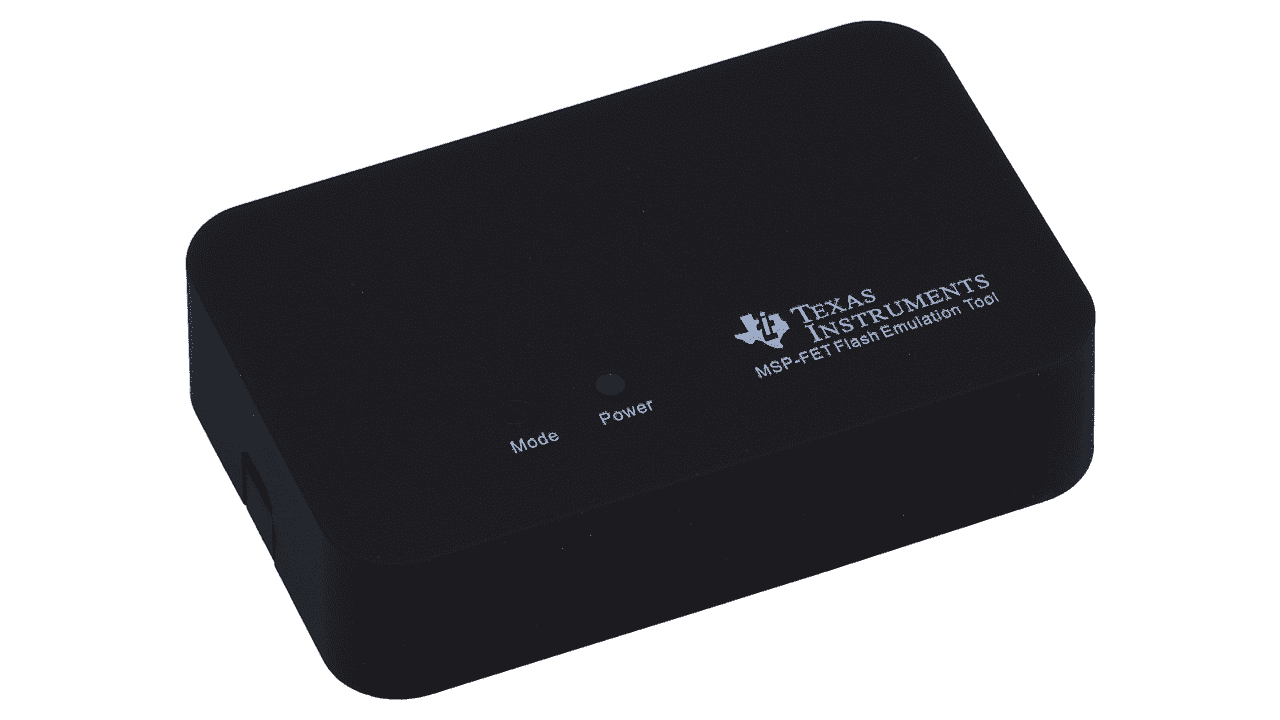
\includegraphics[width=1.0\textwidth]{../Bilder/msp_fet.png}
	\caption{Flash Emulation Tool Programmer and Debugger \Zitat{ti:MSP_FET}}
	\label{fig:msp_fet}
\end{figure}

Der MSP-FET kommuniziert mit dem MSP430-Mikrocontroller typischerweise \"uber standardisierte (Debug-)Schnittstellen wie \textbf{\Abkuerzung{Joint Test Action Group}{JTAG} (Joint Test Action Group)} oder das von Texas Instruments entwickelte \Fachbegriff[Zweidraht-Variante des JTAG-Protokolls, die Pin-Anzahl am Target reduziert und besonders f\"ur platzkritische Anwendungen von Vorteil ist.]{Spy-Bi-Wire}. (\Abkuerzung{Spy-Bi-Wire}{SBW}) \"uber diese Schnittstellen erh\"alt der MSP-FET Zugriff auf das EEM des MSP430FR5729. Wie im vorherigen Abschnitt \ref{Hardware_VS_Software_Breakpoints} dargelegt, ist das EEM f\"ur die Realisierung von Hardware-Breakpoints zust\"andig. Der MSP-FET agiert hierbei als Vermittler, der die vom Entwickler in der \NeuerBegriff{IDE (Integrated Development Environment)} gesetzten Hardware-Breakpoint-Adressen in die entsprechenden Register des EEM schreibt und die vom EEM generierten Haltesignale empf\"angt und an die IDE weiterleitet. Somit ist der MSP-FET unerl\"asslich f\"ur die Konfiguration und Nutzung der limitierten, aber pr\"azisen Hardware-Breakpoint-Ressourcen des Mikrocontrollers. \Zitat[S. 58, Kap. 3.4]{davies:msp430}

Dar\"uber hinaus spielt der MSP-FET eine ebenso gro{\ss}e Rolle f\"ur die Implementierung und Handhabung von Software-Breakpoints. Die F\"ahigkeit, den Speicher des MSP430FR5729 (sowohl RAM als auch das beschreibbare FRAM) zur Laufzeit zu lesen und zu schreiben, ist die Grundvoraussetzung, um Instruktionen mit einer Software-Breakpoint-Routine zu ersetzen. Der Debugger liest \"uber den MSP-FET die urspr\"ungliche Instruktion an der Zieladresse aus, ersetzt diese durch eine Breakpoint-Instruktion und, nach dem Ausl\"osen des Software-Interrupts, stellt er die urspr\"ungliche Instruktion wieder her. Ferner erm\"oglicht der MSP-FET die Steuerung des Programmflusses (Anhalten, Starten, Einzelschrittbetrieb) und den Zugriff auf CPU-Register und Speicherinhalte, was f\"ur die Analyse des Systemzustands an einem Breakpoint unerl\"asslich ist. Das vom Software-Breakpoint ausgel\"oste Interrupt- oder Exception-Signal wird ebenfalls \"uber die Debug-Schnittstelle an den MSP-FET und somit an die Host-Debugger-Software gemeldet. Wie solche Hardware und Software-Breakpoints in der Entwicklungsumgebung aussehen, ist in \Abbildung{CCS_SetBR} zu sehen. Das \glqq H/W\grqq oder \glqq S/W\grqq innerhalb der eckigen Klammern steht wahlweise f\"ur \glqq Hardware\grqq oder \glqq Software\grqq welches von einem \glqq BP\grqq f\"ur \glqq Breakpoint\grqq erg\"anzt wird.

\begin{figure}[h!]
	\centering
	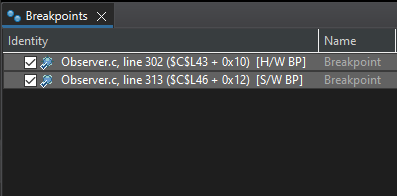
\includegraphics[width=0.75\textwidth]{../Bilder/HW_SW_Breakpoint.png}
	\caption{Code Composer Studio - Breakpoint \"Ubersicht}
	\label{fig:CCS_SetBR}
\end{figure}

Es ist wichtig zu verstehen, dass der MSP-FET prim\"ar die Kommunikationsinfrastruktur und die Low-Level-Zugriffsmechanismen bereitstellt. W\"ahrend er das Setzen von Hardware-Breakpoints direkt \"uber das EEM steuert, stellt er f\"ur Software-Breakpoints die notwendigen Lese-, Schreib- und Kontrolloperationen zur Verf\"ugung. Die eigentliche Logik eines Software-Breakpoints – das hei{\ss}t, welche Instruktion als Breakpoint-Befehl dient, wie die urspr\"ungliche Instruktion gesichert und wiederhergestellt wird sowie der resultierende Trap behandelt wird – muss in der Debugger-Software auf dem Host und gegebenenfalls durch eine minimale Debug-Monitor-Routine auf dem Target implementiert werden, wobei der MSP-FET als Br\"ucke dient. \Zitat[S. 56, Kap. 10]{ti:slau157as, ti:slau654e}

Die Kenntnis der Funktionalit\"aten und der Arbeitsweise des MSP-FET ist somit entscheidend f\"ur die Entwicklung einer robusten Software-Breakpoint-L\"osung. Er definiert die Grenzen und M\"oglichkeiten, wie mit dem Target-System interagiert werden kann, um Breakpoints zu setzen, Zustandsinformationen abzufragen und die Programmausf\"uhrung zu steuern. Die im Folgenden zu entwickelnde Strategie zur Implementierung von Software-Breakpoints muss sich daher eng an den durch den MSP-FET und die Debug-Schnittstelle des MSP430FR5729 gegebenen Rahmenbedingungen orientieren.

\newpage
\subsection{Konzeptionierung von Software-Breakpoints}
\label{sec:KonzeptionierungSoftwareBreakpoints}

Zur Realisierung von Breakpoints existieren mehrere Ans\"atze. Ein bew\"ahrter Einstieg besteht darin, etablierte Debugger und ihre Architektur zu studieren. Im Embedded‑ und Low‑Power‑Bereich kommen beispielsweise Werkzeuge wie \NeuerBegriff{TRACE32}, \NeuerBegriff{M-Core} oder das \NeuerBegriff{MSP-FET} von Texas Instruments zum Einsatz. Diese Debugger setzen Hardware-Breakpoints \"uber spezielle Debug‑Interfaces um und bieten damit eine hohe Zuverl\"assigkeit bei minimaler Eingriffstiefe in das Laufzeitsystem.

Im Gegensatz dazu zielt die hier vorgestellte L\"osung auf eine Abwandlung der Software-Breakpoints ab, die direkt den Programmspeicher manipuliert. Dabei wird, in dieser Implementierung, an der gew\"unschten Halteadresse der originale Maschinenbefehl durch einen Sprungbefehl (Jump) ersetzt, der auf eine speziell implementierte \NeuerBegriff{Breakpoint-Handler}-Routine verweist. Beim Erreichen dieses Befehls wird zun\"achst ein kritischer Abschnitt eingeleitet: Es werden die f\"ur den Prozess relevanten Register (R1 bis R3) – namentlich \Fachbegriff[Ein Register, das die Speicheradresse des derzeitigen Befehls enth\"alt.]{Program Counter} (\Abkuerzung{Program Counter}{PC}), \Fachbegriff[Ein Register, das die Speicheradresse des letzten oder ersten Datenelements im Stack speichert.]{Stack Pointer} (\Abkuerzung{Stack Pointer}{SP}), \Fachbegriff[Register f\"ur eine Reihe von Flags, die von der arithmetisch-logischen Einheit in Abh\"angigkeit der zuletzt durchgef\"uhrten Rechenoperation gesetzt werden.]{Statusregister} (\Abkuerzung{Status Register}{SR}) und \ggf mehrere \NeuerBegriff{General-Purpose-Register (R4 bis R15)} – gesichert und Interrupts deaktiviert, um eine atomare Kontextsicherung zu gew\"ahrleisten \Zitat[S.91, Kap. 4.3]{ti:slau272d}. Anschlie{\ss}end erfolgt der \"ubergang in die Handler-Routine, die das gesamte System bis auf das Observer-Modul blockiert und so das Auslesen und Manipulieren von Speicherinhalten erm\"oglicht.

Nach der Analyse kann der urspr\"ungliche Programmzustand durch das laden der Registers\"atze wiederhergestellt werden. Eine explizite reaktivierung der Interrupts ist daher nicht n\"otig. Der Compiler stellt hierf\"ur \Fachbegriff[Compiler-spezifische, vordefinierte Funktionen, die direkt in optimierten Assemblercode umgesetzt werden.]{Compiler-Intrinsics} bereit wie \Code{\_\_get\_SR()}, \Code{\_\_get\_SP()} und \Code{\_\_set\_interrupt\_state()} \Zitat[S.137, Kap. 6.8.1]{ti:slau132r}. Auf diese Weise wird ein vollst\"andiger Zyklus von Unterbrechung, Inspektion und Fortsetzung des Programmflusses realisiert, ohne dass das Hauptprogramm von dem Observer-Modul tiefgreifender beeinflusst wird.

Vor diesem Hintergrund wird in den folgenden Abschnitten die Konzeptionierung erweiterter Software-Breakpoints im Detail erl\"autert und auf die daf\"ur notwendigen Voraussetzungen eingegangen.

\subsubsection{Verwendung eines Sprungbefehls anstelle einer Trap}
\label{sec:JumpVsTrap}

Wie in Abschnitt \ref{Hardware_VS_Software_Breakpoints} erl\"autert, basieren klassische software-Breakpoints h\"aufig auf sogenannten Trap-Instruktionen. Das Debugging-Framework der Entwicklungsumgebung unterst\"utzt dies unter anderem \"uber die \NeuerBegriff{General Extension Language} (\Abkuerzung{General Extension Language}{GEL}) – ein Makro- und Skriptsystem, das die Initialisierung von Systemen sowie die Steuerung von Debug-Sitzungen erm\"oglicht. Darüber hinaus erlaubt GEL auch das Setzen von Breakpoints, Speicherzugriffe und die Ablaufkontrolle des Programms \Zitat[Kap. 7.7, 7.7.8.6 \& 7.7.8.7]{ti:CCS}.

Für diese Arbeit war es jedoch erforderlich, dass bei Ausl\"osen eines Breakpoints benutzerdefinierte Routinen aus dem Observer-Modul aktiv bleiben und verwendet werden k\"onnen (\Vgl Abschnitt \ref{Interruptgesteuertes_Lesen&Schreiben}). Diese Funktionalit\"aten sind mit dem Standardverhalten von GEL-Traps nicht kompatibel, da sie typischerweise nur auf Debugger-seitige Prozesse abzielen und keine Kontextintegration benutzerdefinierter Routinen auf dem Zielsystem erlauben.

Aus diesem Grund wurde bewusst auf die Verwendung eines Trap-Mechanismus verzichtet und stattdessen ein direkter Sprungbefehl (Jump) auf eine benutzerdefinierte Breakpoint-Handler-Routine implementiert. Dadurch wird sichergestellt, dass das Observer-Modul auch w\"ahrend einer Unterbrechung aktiv bleibt und die Kontrolle \"uber Register- und Speicherzugriffe erhalten bleibt.

\subsubsection{Implementierung erweiterter Software Breakpoints}
\label{sec:ImplementierungSoftwareBreakpoints}

Die Grundidee von Software-Breakpoints besteht darin, an einer Stelle im Programmspeicher, an der ein g\"ultiger Maschinenbefehl (\Fachbegriff[Auch op code oder operation code, ist eine meist in hexadezimaler Schreibweise angegebene Zahl, die die Nummer eines Maschinenbefehls f\"ur einen bestimmten Prozessortyp angibt.]{Opcode}) liegt, diesen tempor\"ar durch einen Sprung auf die Breakpoint-Handler-Routine zu ersetzen. Zun\"achst wird der originale Opcode gesichert, um ihn sp\"ater unver\"andert wieder einsetzen zu k\"onnen. Die Auswahl der Adresse erfordert, dass diese auf ein g\"ultiges Befehlswort ausgerichtet ist und im Stack-Bereich liegt, um Kollisionen auf das Code-Segmenten zu vermeiden. Zudem muss die Interpretation der Adresse und des zu schreibenden Sprungbefehls den aktiven Adressierungsmodus berücksichtigen.

Die Implementierung gliedert sich in folgende Schritte:
\begin{enumerate}
	\item \textbf{Adressvalidierung:} Pr\"ufen, ob die Zieladresse auf vier Byte ausgerichtet ist und im Stack liegt.
	  
	\item \textbf{Kontext-Sicherung:} In einem kritischen Abschnitt werden PC, SP, SR und alle modifizierten Register in einem Puffer abgelegt. Hierbei ist zu beachten, dass die Breite des PC vom Adressierungsmodus abh\"angt, worauf entsprechend r\"ucksicht genommen werden muss. \Zitat[S. 97, Kap. 4.4]{ti:slau272d}
	
	\item \textbf{Ersetzen des Opcodes:} Der Original-Opcode (vier Byte) wird durch den vier-Byte-Sprungbefehl (zwei Byte f\"ur den Instruction-Code, zwei Byte f\"ur die Zieladresse der Handler-Routine) \"uberschrieben. \Zitat[S.161, Kap. 4.6.2.28]{ti:slau272d}
	
	\item \textbf{Ausf\"uhrung des Breakpoint-Handlers:} Beim Eintreten des Breakpoint-Opcodes springt der PC in die Handler-Routine, die das System an weiterer Ausf\"uhrung hindert und stattdessen das Observer-Modul f\"ur weitere Debug-Schritte aktiv h\"alt.
	
	\item \textbf{Kontext-Wiederherstellung:} Nach Abschluss der Debug-Aktion werden alle Register und der urspr\"ungliche Opcode wiederhergestellt, bevor der normale Programmablauf fortgesetzt wird.
\end{enumerate}

Diese Vorgehensweise stellt die R\"uckkehr zum urspr\"unglichen Systemzustand – einschlie{\ss}lich des Originalen-Opcodes – sicher und garantiert die Konsistenz des Programms.

Um die im vorigen Abschnitt \ref{sec:KonzeptionierungSoftwareBreakpoints} skizzierten Konzepte robust umzusetzen, sind die im n\"achsten Abschnitt, technischen Details wie Instruktionsl\"angen und Speicher-Alignment, zu betrachten.\AI

\subsubsection{Instruktionsl\"angen, Speicher-Alignment und Adress-Modi}
\label{sec:TechnischeUmsetzunSoftwareBreakpoints}

Die Manipulation von Befehlen im Stack ist hoch kritisch, da das Hauptprogramm keine Kenntnis vom Observer-Modul hat und eine falsche Adressierung, unterschiedlichen Adressierungs-Modi oder unvollst\"andige Opcode-substituierung zu undefiniertem Verhalten f\"uhren kann. Drei zentrale Aspekte sind dabei zu beachten:

\begin{itemize}
	\item \textbf{Speicher-Alignment:} MSP430-Instruktionen sind grundsätzlich an geraden Speicheradressen ausgerichtet. Vor jedem Schreib- oder Lesezugriff muss daher sichergestellt werden, dass die Zieladresse eine gerade Adresse ist. Zugriffe auf ungerade Adressen können zu undefiniertem Verhalten führen, sofern keine Fehlerbehandlung erfolgt. Darüber hinaus sind Adressen, die in der Mitte eines Opcodes liegen, ungültig und dürfen nicht als Breakpoint oder adressiert werden.
	
	\item \textbf{Opcode-L\"angen:} W\"ahrend einzelne Maschinenbefehle in der Regel zwei bis vier Bytes belegen, k\"onnen komplexe Instruktionen – etwa \Code{CMP.B} – bis zu sechs Bytes lang sein, wie in \Abbildung{DisassemblyOpcodeLaengen} zu sehen. \Zitat[S.165, Kap. 4.6.2.32]{ti:slau272d} Diese Variabilit\"at erschwert das gezielte \"Uberschreiben von genau vier Byte, die f\"ur die Jump-Instruktion einschlie{\ss}lich Zieladresse ben\"otigt werden. Unter diesen Randbedingungen besteht die Gefahr, dass entweder zu viele oder zu wenige Bytes \"uberschrieben werden, was zu ung\"ultigen oder unbeabsichtigten Instruktionen f\"uhren kann.
	
	\item \textbf{Adressierungs Modus:} Der Speicher, im Umfang von einem Megabyte, kann \"uber sieben unterschiedliche arten Adressiert werden. Wahlweise kommen 16 oder 20-Bit Adressen zum Einsatz. Diese Variabilität der Adressierungsmodi und die damit einhergehenden unterschiedlichen Adressbreiten haben tiefgreifende Konsequenzen.\Zitat[S. 97, Kap. 4.4]{ti:slau272d}
\end{itemize}

\begin{figure}[h!]
	\centering
	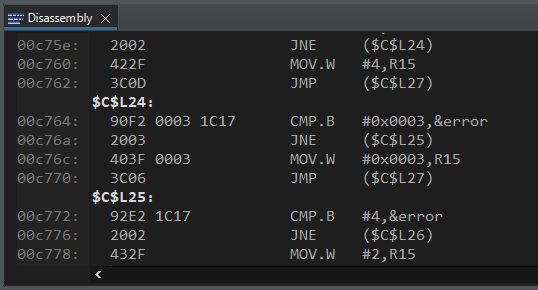
\includegraphics[width=0.75\textwidth]{../Bilder/OpcodeLaengen.png}
	\caption{Code Composer Disassembly Modus - Opcode l\"angen}
	\label{fig:DisassemblyOpcodeLaengen}
\end{figure}

Das Sichern und Wiederherstellen von Registern und des Originalen Opcodes reicht daher nicht aus, insbesondere angesichts den variablen Instruktionsl\"angen und komplexer Adressierungsmodi. 

Die gr\"o{\ss}e der Opcodes h\"angt von folgenden Parametern ab. Die Grundlegende l\"ange einer Instruktion des MSP430 liegt bei zwei Byte. Darin ist die Operation, wie beispielsweise \Code{MOV.W}, sowie die Register- und Adressierungsart kodiert. Unterschiedliche Adressierungen von Operanden \"uber Adressierungsmodi wie \glqq \Fachbegriff[Operand ist direkt in der Instruktion enthalten – also ein fester Wert, nicht aus dem Speicher.]{Immediate}\grqq , \glqq \Fachbegriff[Operand befindet sich an einer feste Speicheradresse.]{Absolute} \grqq oder \glqq \Fachbegriff[Operand ist nicht direkt gegeben, sondern steht an der Adresse, die ein Register enth\"alt.]{Indirect}\grqq, haben zur Folge, dass die Adressen oder Konstanten zus\"atzlich als \Fachbegriff[Synonym f\"ur 2 Byte gro{\ss}e Datenbreite]{Word} (2 Byte) oder \Fachbegriff[Synonym f\"ur 4 Byte gro{\ss}e Datenbreite]{extended Word} (4 Byte) kodiert werden. \Zitat[S. 97, Kap. 4.4]{ti:slau272d}

Ein Beispiel hierzu, woraus sich der 6-Byte lange Opcode, zum Vergleichen des Speicherinhalts des Registers \glqq \&error\grqq  mit dem Hexadezimalen Wert \glqq 0x0003\grqq, aus \Abbildung{DisassemblyOpcodeLaengen} zusammensetzt:
\\\textbf{\Code{CMP.B \#0x0003, \&error}}
\begin{itemize}
	\item \textbf{1 Byte} Opcode f\"ur \Code{CMP.B}
	\item \textbf{1 Byte} Modus f\"ur Quell-Operand und Ziel-Operand (Immediate -> Absolute)
	\item \textbf{2 Byte} Immediate-Wert f\"ur Konstante \glqq 0x0003\grqq
	\item \textbf{2 Byte} Absolute-Adresse f\"ur Label \glqq \&error\grqq
\end{itemize}
\Zitat[S. 147, Kap. 4.6.2.14 \& S. 112, Kap. 4.4.7 \& S. 108, Kap. 4.4.4]{ti:slau272d}

Diese Analyse verdeutlicht die komplexit\"at der Manipulation und Wiederherstellung von Instruktionen im Stack. Eine Kopie des Stacks schafft dabei eine sichere Umgebung, in welcher der bestehende Opcode Manipuliert wird. Hierbei muss die Kopie die unterschiedlichen Adressformate und die potenziell im Stack gespeicherten, modusabh\"angigen Zeiger korrekt abbilden oder transformieren. Dies garantiert ein sicheres zur\"uckkehren in die Hauptroutinen, sowie eine Robuste Ausf\"uhrung der Funktion zum verarbeiten der \ggf mehreren Breakpoints.

Dies erschwert die Umsetzung und erh\"oht die Komplexit\"at der Routine erheblich, wodurch Timing und Konsistenz gef\"ahrdet werden. Im anschlie{\ss}enden Fazit werden die gewonnenen Erkenntnisse bewertet, offene Fragestellungen skizziert und ein Ausblick auf weiterf\"uhrende Arbeiten gegeben.

\subsection{Fazit zur Umsetzung von Software Breakpoints}
\label{sec:FazitSoftwareBreakpoints}

Die Realisierung von Software-Breakpoints auf dem Low‑Power‑Mikrocontroller MSP430FR5729 erfordert ein tiefgehendes Verst\"andnis der Prozessor‑Architektur, der Instruktionsformate, der vielf\"altigen Adressierungs-Modi und ihrer Auswirkungen auf die Speicherverwaltung und der nebenl\"aufigen Abl\"aufe im System. Die Analyse der Problemstellung hat ergeben, dass unter anderem kritische Bereiche atomar bearbeitet, Register und Stack-Zust\"ande zuverl\"assig gesichert und Intrinsics korrekt eingesetzt werden m\"ussen. Zudem sind umfangreiche Funktionen zur \"uberwachung und Protokollierung des Systemzustands zu implementieren.

Die erwartete komplexit\"at inklusive der Anforderungen an Robustheit, Echtzeitf\"ahigkeit und m\"oglichst geringem Eingriff in den Betrieb \"uberschreitet den Rahmen einer \"ublichen Bachelorarbeit. Eine vollst\"andige, ausgereifte Implementierung w\"are mit dem Umfang einer Masterarbeit oder vergleichbarer Forschungsarbeiten m\"oglich. Dennoch bildet dieses Thema eine exzellente Grundlage f\"ur weiterf\"uhrende Arbeiten in den Bereichen eingebettete Echtzeitsysteme und Debugging‑Technologien, insbesondere in Bezug auf Architekturen mit flexiblen, aber komplexen Speicheradressierungsmechanismen.

